\subsection*{Exercise 1}

\subsubsection*{(a)}
The basis vector is a vector that starts from an atom and goes to the closer atom of the same type. For example we can choose the leftmost $Na^+$ as the origin and we draw a vector until the second $Na^+$. The base unit cell is made of a couple $Na^+ + Cl^-$

\subsubsection*{(b)}
Let us take a $Na^+$ atom at position x and suppose that the chain is infinitely long both at the left and at the right. Each $Cl^-$ atom exerts an attractive force ( negative potential) on the $Na^+$ atom and each other $Na^+$ exerts a repulsive one (positive potential). Hence, in atomic units
$$V(x) = 2 \cdot \left[\frac{1}{a} - \frac{1}{2a} + \frac{1}{3a} - \dots \right]= \frac{2}{a }\sum_{n=1}^{+\infty} \frac{(-1)^{n+1}}{n} = \frac{2 \ln 2}{a}$$
Then the Madelung constant is $M = 2 \ln 2$ 

\subsubsection*{(c)}
A consequence of the presence of only a finite number of atoms is that symmetry is broken: each atom has now a different number of atoms on its right and left (except for the central one) and this 
effect becomes smaller as the number of atoms increases (more atoms can be approximated as "centrals"). Remember that the Madelung constant is a geometrical factor related to the energy per molecule in the crystal. 
One can now proceed in two different ways which will be equivalent in the limit of large $N$ as shown in figure \ref{fig:Madelung_constant_Natoms}.
\begin{enumerate}
    \item Neglect border effects and consider each atom as "central". This can be reasonable since the Coulomb potential decreases rapidly with the atom index. In this case the total energy of the lattice is approximately
    $U = NU_i$ where
    $$ U_i = 2\sum_{n=1}^{N/2}\frac{(-1)^n}{n a} = \frac{\alpha}{a}$$
    and $\alpha$ is the Madelung constant.
    \item Consider the border effects and the fact that not all atoms have the same energy. In this case the value of the Madelung constant would depend on the chosen atom, so we calculate an "average" Madelung constant by calculating the average energy of each molecule in the crystal as $V_{tot}/N_{molecules} = V_{tot}/(N/2)$ and use that expression to evaluate the Madelung constant. \\
        The total energy of the system can be computed as a sum over all the particles' interactions. If we begin the chain with a $Na^+$ atom, the charge of the $n-th$ atom in the chain is in atomic units $(-1)^n$, hence
        $$U = \frac{1}{2} \sum_{i \neq j} \frac{(-1)^i(-1)^j}{r_{ij}} = \frac{1}{2} \sum_{i \neq j} \frac{(-1)^{i+j}}{|i-j| \, a} =
        \frac{N\alpha}{2a}$$
        and this provides an estimation for the Madelung constant $\alpha$.
\end{enumerate} 
The Madelung constant for both models as a function of the number of atoms is plotted in figure \ref{fig:Madelung_constant_Natoms}.
\begin{figure}[h]
    \centering 
    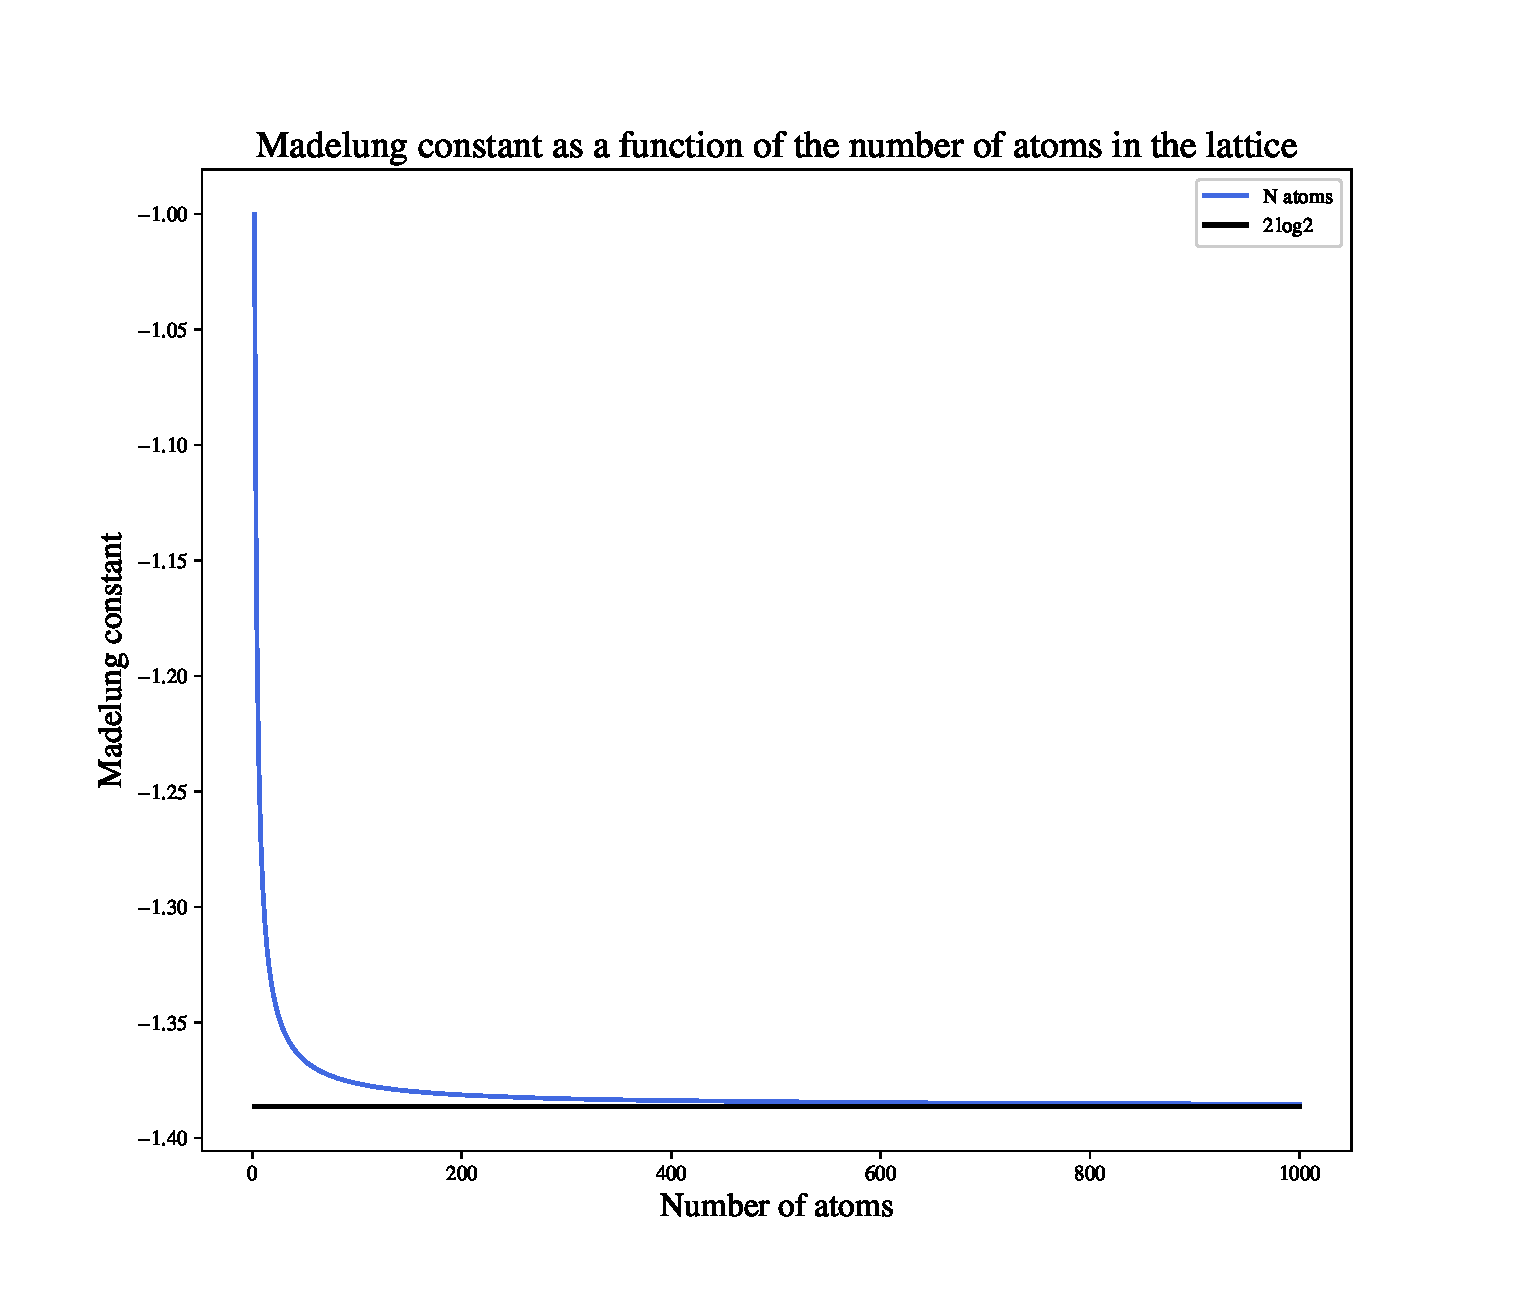
\includegraphics[scale=0.7]{figures/madelung.eps}
    \caption{Madelung constant as a function of the number of atoms}
    \label{fig:Madelung_constant_Natoms}
\end{figure}

\subsubsection*{(d)}
To simply the calculation we here neglect border effects and calculate the energy of the crystal as the sum of the electrostatic energy and the Pauli repulsion energy (nearest neighbour only). Let us denote with $a$ the interatomic distance of the lattice. Each atom in the center of the crystal has energy equal to
\begin{equation*}
    U_i(a) = 2 \sum_{i \neq j}U_{ij}(a) = 2\left(\lambda e^{-a/\rho} - \sum_{i \neq j}\frac{1}{r_{ij}}\right) = 
    2\left(\lambda e^{-a/\rho} - \sum_{n=1}^{N/2}\frac{(-1)^{n}}{n}\right)
\end{equation*}
The equilibrium distance can be obtained by searching the minimum of the energy per atom
\begin{equation*}
    \frac{\partial U_i}{\partial a} = 0
\end{equation*}
The equation can be solved numerically and the the result is reported in figure \ref{fig:NaCl_constant}

\begin{figure}
    \centering 
    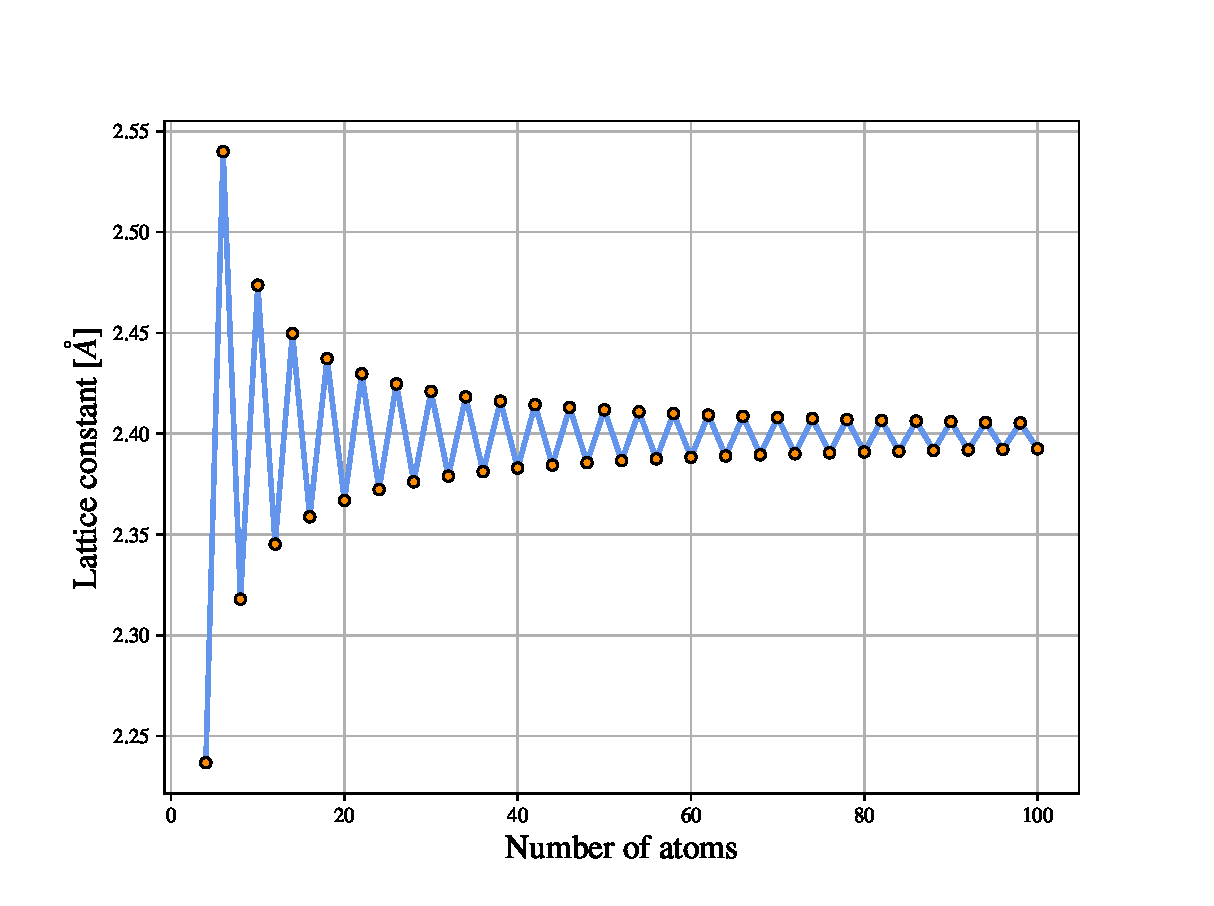
\includegraphics[scale=0.7]{figures/NaCl_constant.eps}
    \caption{}
    \label{fig:NaCl_constant}
\end{figure}

\subsection*{Exercise 2}
\subsubsection*{(a)}
$$N = 12 \cdot \frac{1}{6} + 2 \cdot \frac{1}{2} + 3 \cdot 1 = 6$$
\subsubsection*{(b)}
Let us consider the tetrahedon composed by two adiacent atoms in the lowest layes, the central atom in the lowest layer and the closest atom in the middle layer.
Since the tetrahedon is regular, all the sides are of the same length. The distance $x$ of the projection of the middle layer point to the lowest layer from a vertex of the triangle is 
$$x = \frac{a}{2}\frac{1}{\cos\frac{\theta}{2}} = \frac{a}{\sqrt{3}}$$
Hence the  height of the middle point is 
$$h = \sqrt{a^2 - \frac{a^2}{3}} = \sqrt{\frac{2}{3}}a$$ hence the height of the base cell is $c = 2h = \sqrt{8/3}a$ and the $c/a$ ratio is $\sqrt{8/3}$.
\subsubsection*{(c)}
Just substitute $a=2r$ and calculate directly from the general formula.

\subsection*{Exercise 3}
Let us choose a set of parallel planes. From this set we choose the plane closer to the origin. The idea is to calculate the distance between planes as the distance from the origin to this plane. Let us suppose that the plane intersects the $x,y,z$ axes of a cube respectively in positions $x_1, x_2, x_3$: the crystal requires that 
\begin{gather*} 
    x_1 = n_1 a \\
    x_2 = n_2 a \\
    x_3 = n_3 a
\end{gather*}
where $a$ is the lattice constant. \\
The Miller indices of the plane are defined as 
$$(hkl) \equiv (h, k, l) \equiv C \left(\frac{1}{n_1 a}, \frac{1}{n_2 a}, \frac{1}{n_3 a}\right)$$
where $N$ is a constant that guarantees that $(hkl)$ is a set of integer numbers (the minimum integers that keeps the reciprocal proportionality). Without loss of generalisation we can assume $N$ to be equal to $1$; in fact, otherwise, $N$ would be a common multiple of $n_1, n_2, n_3$ and we can return to the case above defining $n_k' = n_k/N \quad \forall k$. \\
If one takes the general equation of a plane
\begin{equation*} 
    ax + by + cz + d = 0
    \label{eq:implicit_plane_general}
\end{equation*}
it is possible to define the distance of the plane $\pi$ to a point $P$ via the formula
\begin{equation} 
    d(P, \pi) = \frac{|ax_p + by_p + cz_p + d|}{\sqrt{a^2 + b^2 + c^2}}
    \label{eq:point_plane_distance}
\end{equation}
Equation \ref{eq:implicit_plane_general} can be rewritten as
\begin{equation}
    \frac{x}{c_1} + \frac{y}{c_2} + \frac{y}{c_3} = 1
\end{equation}
and in this form the parameters $c_1, c_2, c_3$ assume the geometrical significance of intercepts of the axes (just check by setting $x,y,z$ equal to $0$ in couples). This particularly useful in our case, since we can write the equation of our plane as
\begin{equation*}
    \frac{x}{n_1 a} + \frac{y}{n_2 b} + \frac{y}{c_3} = 1
\end{equation*}
and using \ref{eq:point_plane_distance} for the origin 
$$d(O, \pi) = \frac{1}{\sqrt{(\frac{1}{n_1 a})^2 + (\frac{1}{n_2 a})^2 + (\frac{1}{n_3 a})^2}}$$
or
$$d(O, \pi) = \frac{a}{\sqrt{h^2 + k^2 + l^2}}$$

\subsubsection*{Exercise 4}

\subsubsection*{(a)}
\begin{enumerate}
    \item (010)
    \item (210)
    \item (010)
    \item (120)
    \item (010)
    \item (100)
\end{enumerate}

\subsubsection*{(c) and (d)}
Diffraction occurs if the von Laue condition is satisfied, that its
$$2 \ve k \cdot \ve G + G^2 = 0$$
\begin{enumerate}
    \item if $\ve k \cdot \ve G > 0$ the above expression is always positive, hence the result is trivial
    \item if $\ve k \cdot \ve G < 0$ then 
        $$ \ve k \cdot \ ve G = - k_g G > - \frac{G^2}{2}$$
        hence
        $$2 \ve k \cdot \ve G + G^2 > -2 \frac{G^2}{2} + G^2 = 0$$

\end{enumerate}


\section*{Exercise 7}

\subsubsection*{(a)}
Suppose that we have N sites, and n of them are vacancies. Let us calculate the configurational entropy of the system as
$$S = k_B \ln\omega$$
If we imagine the sites as a 1D sequence we can calculate the number of possible ways to 
combine $n$ objects of type $A$ with $N-n$ objects of type $B$. In this case
$$\omega(N, n) = \frac{N!}{n!(N-n)!}$$
Let us take the logarithm of this expression and use the Stirling's approximation
$$\ln \omega = \ln(N!) - \ln(n!) - \ln((N-n)!) \approx N \ln N - n \ln n - (N-n)\ln(N-n)$$
If temperature and pressure are constant, then the equilibrium state of the system is the one that minimizes the free energy
$$G = H - TS = U + pV - TS$$
Since the free energy of the lattice without vacancies is a constant, we can restrict the analysis to minimize the vacancies contribution only which practically
means that we can minimize $$\left(\Delta G\right)_\text{vac} = G_\text{tot} - G_\text{no vacancies}$$
If we assume pressure and temperature constant the expression becomes
$$\Delta G = nE_f + npV_f- T\Delta S$$ 
where $E_f$ is the energy required to remove a site and $V_f$ is the volume of a site.
We can search for the minimum in this way 
$$ 0 = \frac{d \Delta G}{dn} = E-f + pV_f - k_B\ln\left(\frac{N-n}{n}\right)$$
$$\frac{E_f}{k_BT} = \ln\left(\frac{N-n}{n}\right)$$
or
$$\frac{n}{N-n} = \exp\left(-\frac{E_f}{k_B T}\right) \, \exp\left(-\frac{pV_f}{k_B T}\right)$$
and if $n << N$
\begin{equation}
    c_v = \frac{n}{N} = e^{-E_f/k_B T} \, e^{-p V/k_B T}
    \label{eq:concentration}
\end{equation}
Pressure is just a particular case of the stress (it is just the case in which the force is orthogonal to the surface). Hence equation \ref{eq:concentration} can 
be generalised to an applied stress with module $\sigma$
\begin{equation*}
    c_v = \frac{n}{N} = e^{-E_f/k_B T} \, e^{-\sigma V/k_B T}
\end{equation*}

\subsubsection*{(b)}
The formation energy is the energy required to move an atom from the site to the surface of the lattiec and in equation \ref{eq:concentration} is represented by $E_f$.
When an atom is removed the lattice get deformed and it generates an internal stress. The deformation causes a variation in the volume and the difference between the final state of the 
system (after moving the atom) and the initial state is the formation volume.